\chapter{불확정성, 에렌페스트 정리, 그리고 고전적 극한}

\section{선형 해밀토니안의 미해결 문제}

모형
\begin{equation}
H=cP
\label{eq:l10-linear-hamiltonian}
\end{equation}
의 파동묶음은 모양을 바꾸지 않고 평행이동하기 때문에 유용했다. 하지만 이 모형은 중대한 경고도 담고 있다. 운동량은 양수일 수도 음수일 수도 있으므로, 같은 식이 한 평면파에는 양의 에너지를, 다른 평면파에는 음의 에너지를 부여한다.
\begin{equation}
\psi_p(x)=e^{ipx/\hbar},
\qquad
E(p)=cp.
\end{equation}
물리적 입자가 음의 에너지 상태를 임의로 많이 차지할 수 있다면, 빈 공간은 최저 에너지 상태가 아니다. 전체 에너지는 보존하면서 양의 에너지 양자를 만들고 그에 상응하는 음의 에너지를 새 입자에 부여하여 진공의 에너지를 한없이 낮출 수 있다.

\begin{classroomqa}
\audiencequestion{음의 에너지 가지가 단지 에너지의 기준점을 특이하게 정한 것 이상인 이유는 무엇인가요?}
\lecturerresponse{모든 에너지에 같은 상수를 더하는 것은 문제가 되지 않는다. 에너지 스펙트럼이 아래로 한정되지 않는 것은 다른 문제다. 양의 에너지 입자가 에너지 차이를 가져가는 동안 더 낮은 에너지 상태를 계속 채울 수 있다면 안정한 바닥 상태가 존재하지 않는다. 안정성을 위해서는 진공을 기준으로 에너지에 하한이 있어야 한다.}
\end{classroomqa}

\begin{figure}[htbp]
\centering
\includegraphics[width=0.88\textwidth]{lecture_10_figure_01.png}
\caption{선형 해밀토니안과 평면파 고유함수에서는 \(p<0\)일 때 음의 에너지 가지가 드러난다.}
\lectureframe{00:04:35}
\end{figure}

디랙의 역사적 해법은 페르미온에는 통했다. 페르미온은 배타 원리를 따른다. 즉, 서로 동일한 페르미온 두 개가 같은 일입자 상태를 차지할 수 없다. 음의 에너지 상태를 모두 채운다고 생각해 보자. 그 상태들이 모두 차면, 배타 원리에 따라 다른 페르미온이 그 영역으로 떨어질 수 없다. 가득 찬 집합에서 생긴 빈자리는 반입자처럼 작용한다.

이 논증은 음의 에너지를 가진 보손을 구제하지 못한다. 보손은 한 상태를 임의의 수만큼 차지할 수 있으므로, 음의 에너지를 가진 보손 모드는 한도 없이 채워질 수 있다. 과거의 바다 모형은 반입자 개념에 이르게 된 역사적 경로로 보는 것이 가장 적절하다. 현대 양자장론에서는 물리적 진공을 관측 가능한 음의 에너지 전자의 문자 그대로의 바다로 취급하지 않고 입자와 반입자를 설명한다. 여기서 필요한 요점은 더 제한적이다. 이 장난감 해밀토니안은 안정한 입자 이론의 완전한 모형이 아니다.

고정된 속력으로 움직이는 페르미온 입자의 1차원 캐리커처인 이 모형은 디랙의 아이디어가 관련되었던 중성미자 문제를 어렴풋이 보여 준다. 하지만 광자 이론으로 쓸 수는 없다. 광자는 보손이므로, 배타 원리로 광자의 음의 에너지 상태를 채워 막을 수 없다.

\begin{classroomqa}
\audiencequestion{배타 원리는 페르미온 구성은 안정화할 수 있지만 보손 구성은 왜 안정화하지 못하나요?}
\lecturerresponse{페르미온 상태는 한 번 채우면 더는 채울 수 없다. 보손 상태에는 그런 점유 상한이 없으므로, 음의 에너지를 가진 보손 모드에서는 에너지가 계속 한없이 낮아질 수 있다.}
\end{classroomqa}

\paragraph{이제까지 강의에서 다룬 내용.}
이번 학기에는 양자역학의 기초 대부분과 몇 가지 의도적으로 단순화한 계를 다뤘지만, 응용은 거의 다루지 않았다. 특히 조화 진동자조차 아직 배우지 않았다. 이는 끝이 아니라 경계를 나타낸다. 다음에는 상대론과 장론을 공부하고, 그 뒤 조화 진동자와 이를 바탕으로 하는 다른 구조를 살펴보기 위해 양자역학으로 돌아와야 한다. 앞서 얽힘을 다룬 논의에 꾸준히 관심이 모였다는 점은 기초부터 살펴보는 경로가 왜 유익했는지도 보여 준다.

이 관점에서 보면 미해결 문제는 정리된다. 이제 핵심은 파동함수와 불확정성, 그리고 양자 시간 발전과 고전역학의 관계다. 목표는 가능한 한 가장 일반적인 시간 발전 방정식이 아니라, 원래 Schr\"odinger가 쓴 특수한 위치 공간 방정식이다.

\section{파동함수와 완전 가환 좌표}

직선 위를 움직이는 입자 하나의 위치 공간 파동함수는
\begin{equation}
\psi(x)=\braket{x}{\psi},
\end{equation}
입자를 \(x\) 근처에서 발견할 확률진폭이다. 운동량 공간 파동함수는
\begin{equation}
\widetilde{\psi}(p)=\braket{p}{\psi}.
\end{equation}
이다. 두 파동함수는 같은 추상 상태를 서로 다른 기저로 나타내며 푸리에 변환으로 연결된다.
\begin{align}
\psi(x)
&=
\int_{-\infty}^{\infty}
\frac{dp}{\sqrt{2\pi\hbar}}\,
\widetilde{\psi}(p)e^{ipx/\hbar},
\label{eq:l10-fourier-forward}\\
\widetilde{\psi}(p)
&=
\int_{-\infty}^{\infty}
\frac{dx}{\sqrt{2\pi\hbar}}\,
\psi(x)e^{-ipx/\hbar}.
\label{eq:l10-fourier-inverse}
\end{align}

\begin{figure}[htbp]
\centering
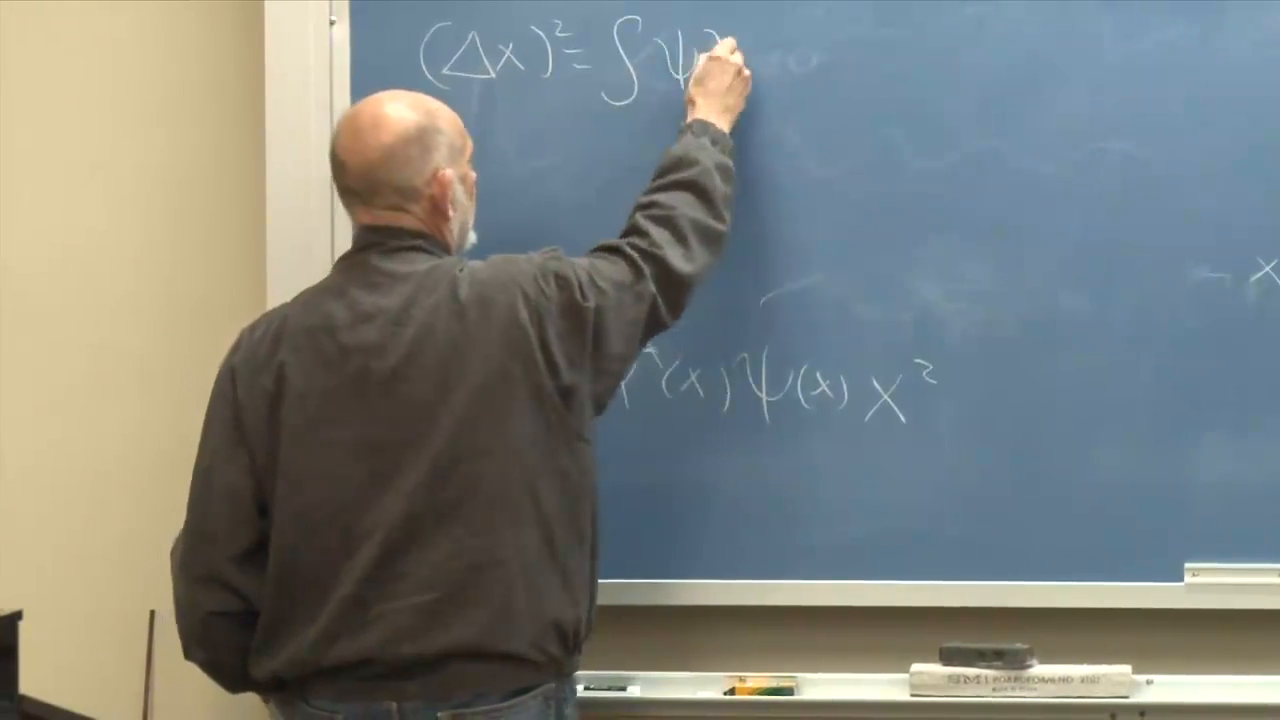
\includegraphics[width=0.88\textwidth]{lecture_10_figure_02.png}
\caption{위치 파동함수와 운동량 파동함수는 하나의 상태를 서로 다른 두 연속 기저에 투영한 것이다.}
\lectureframe{00:09:05}
\end{figure}

공간이 2차원일 때 \(X\)와 \(Y\)는 가환하므로, 공통 고유기저를 두 좌표로 표시할 수 있고 파동함수는 \(\psi(x,y)\)가 된다. 이런 가환성이 추상 공리만으로 강제되는 것은 아니다. 이는 통상적인 공간에 대한 양자역학적 설명이 실험적으로 성공했다는 사실의 일부다. 3차원에서 \(N\)개의 입자에 대해서는
\begin{equation}
\psi(\mathbf{x}_1,\ldots,\mathbf{x}_N)
\end{equation}
이 파동함수는 구성 공간 위의 함수이지, 각 입자에 독립적으로 붙어 있는 3차원 파동이 아니다. 따라서 거시적 계에는 엄청나게 많은 좌표가 필요할 수 있다.

\begin{classroomqa}
\audiencequestion{서로 다른 공간 좌표의 가환성은 양자역학에서 자동으로 따라 나오나요?}
\lecturerresponse{아니다. 추상적 틀은 다양한 관측량 대수들을 허용한다. 서로 다른 데카르트 위치 성분들이 가환한다는 사실은 통상적인 공간에 있는 입자들의 양자역학에 관한 경험적 구조 사실이다.}
\end{classroomqa}

모든 좌표를 푸리에 변환하여 모든 운동량의 함수인 파동함수를 얻을 수도 있고, 일부 변수만 변환할 수도 있다. 표현은 기저를 선택하는 것이지 물리적 상태를 바꾸는 것이 아니므로, 혼합 표현도 타당하다.

\section{불확정성이 측정하는 것}

불확정성 원리의 가장 기본적인 형태는 푸리에 쌍에서 곧바로 따라 나온다. 운동량이 확정된 상태는 절댓값이 일정하고 위치에 국소화되지 않은 평면파다. 위치에 뚜렷하게 국소화된 상태에는 많은 운동량 성분이 필요하다. 더 일반적으로 푸리에 쌍의 한쪽 폭을 좁히면 다른 쪽 폭은 넓어진다.

\begin{figure}[htbp]
\centering
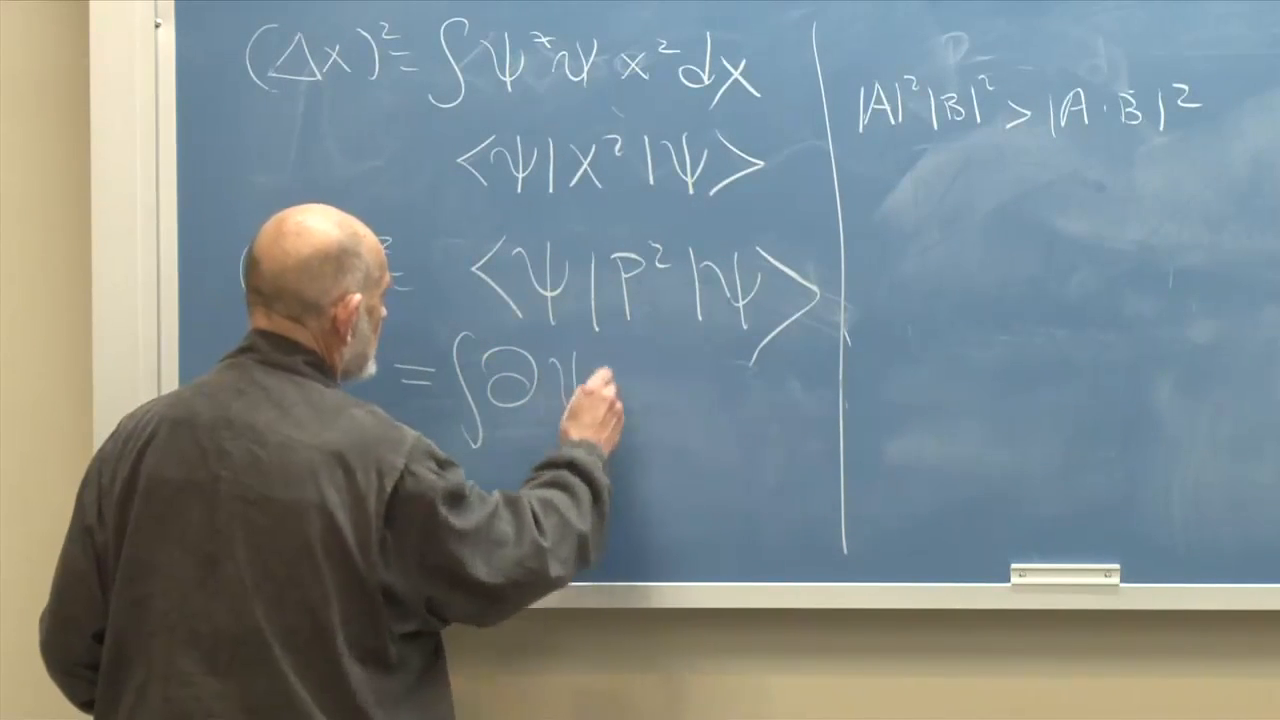
\includegraphics[width=0.88\textwidth]{lecture_10_figure_03.png}
\caption{역수인 운동량 표현에서 위치 분포를 국소화하려면 넓은 범위의 평면파를 중첩해야 한다.}
\lectureframe{00:14:45}
\end{figure}

이 진술을 정량화하려면 먼저 일반적인 관측량 \(Q\)를 생각하자. 정규화된 상태에서 그 기댓값은
\begin{equation}
\expect{Q}=\bra{\psi}Q\ket{\psi}.
\end{equation}
이다. 분산은
\begin{equation}
(\Delta Q)^2
=
\expect{\bigl(Q-\expect{Q}\bigr)^2}
=
\expect{Q^2}-\expect{Q}^2.
\label{eq:l10-general-variance}
\end{equation}
이다. 불확정성 \(\Delta Q\)는 이 분산의 양의 제곱근이다.

위치의 경우 먼저 원점을 옮겨 \(\expect{X}=0\)가 되도록 할 수 있다. 그러면
\begin{equation}
(\Delta x)^2
=
\expect{X^2}
=
\int_{-\infty}^{\infty}
dx\,|\psi(x)|^2x^2.
\label{eq:l10-position-variance}
\end{equation}
\(\expect{X}\)에서는 양수 기여분과 음수 기여분이 서로 상쇄되지만, \(\expect{X^2}\)에서는 서로 더해진다. 따라서 확률분포가 넓을수록 분산은 커진다.

\begin{figure}[htbp]
\centering
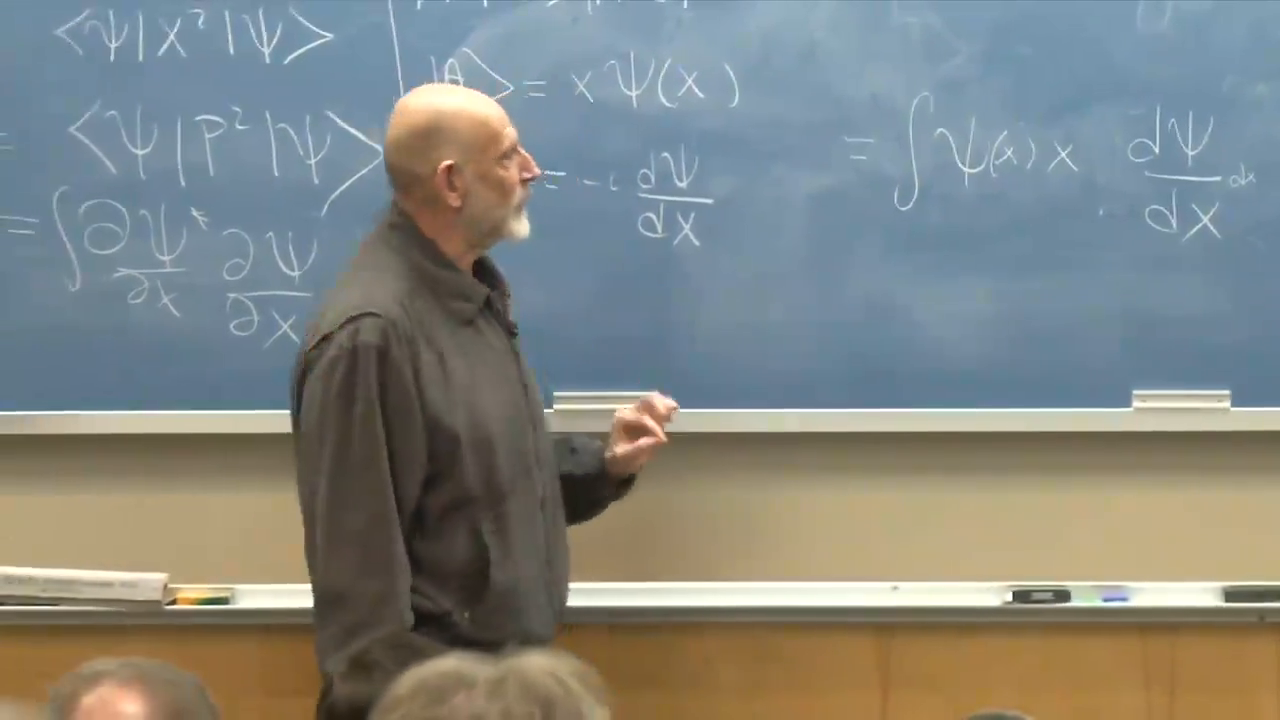
\includegraphics[width=0.88\textwidth]{lecture_10_figure_04.png}
\caption{평균을 0으로 옮기면 위치 분산은 \(x^2\)에 확률을 가중하여 적분한 값이다.}
\lectureframe{00:20:50}
\end{figure}

\(\expect{X^2}\)와 \(\expect{X}^2\)의 차이는 필수적이다. 0을 중심으로 대칭인 분포는 \(\expect{X}=0\)이지만, 원점에 집중되어 있지 않다면 여전히 \(\expect{X^2}>0\)이다.

운동량 분산은 운동량 공간에서 바로 정의할 수 있다.
\begin{equation}
(\Delta p)^2
=
\int_{-\infty}^{\infty}
dp\,|\widetilde{\psi}(p)|^2
\bigl(p-\expect{P}\bigr)^2.
\end{equation}
증명에는 위치 공간에서 계산하는 편이 더 유용하다. 평균 운동량을 0으로 옮기고 다음을 이용하자.
\begin{equation}
P=-i\hbar\frac{d}{dx},
\qquad
P^2=-\hbar^2\frac{d^2}{dx^2}.
\end{equation}
그러면
\begin{equation}
(\Delta p)^2
=
\expect{P^2}
=
-\hbar^2
\int_{-\infty}^{\infty}
dx\,\psi^*(x)\frac{d^2\psi}{dx^2}.
\label{eq:l10-momentum-variance-second}
\end{equation}

\begin{classroomqa}
\audiencequestion{위치 공간에서 분산을 나타내는 식이 음수 부호로 시작하는데도 분산이 어떻게 양수일 수 있나요?}
\lecturerresponse{그 부호에 곱해지는 적분은 양수가 아닙니다. 부분적분을 하면 미분 연산자 하나가 \(\psi^*\)에 작용하게 되어 음수 부호가 하나 더 생기고, 결과는 절댓값의 제곱을 적분한 형태가 됩니다.}
\end{classroomqa}

무한대에서 충분히 빠르게 감소하는 파동함수에 대해서는
\begin{equation}
\int f\,g'\,dx
=
\left[fg\right]_{-\infty}^{\infty}
-
\int f'g\,dx,
\end{equation}
경계항이 사라진다. 이를 식~\eqref{eq:l10-momentum-variance-second}에 한 번 적용하면
\begin{equation}
(\Delta p)^2
=
\hbar^2
\int_{-\infty}^{\infty}
dx\,
\frac{d\psi^*}{dx}
\frac{d\psi}{dx}
=
\hbar^2
\int_{-\infty}^{\infty}
dx\,
\left|\frac{d\psi}{dx}\right|^2
\geq 0.
\label{eq:l10-momentum-variance-positive}
\end{equation}

\begin{figure}[htbp]
\centering
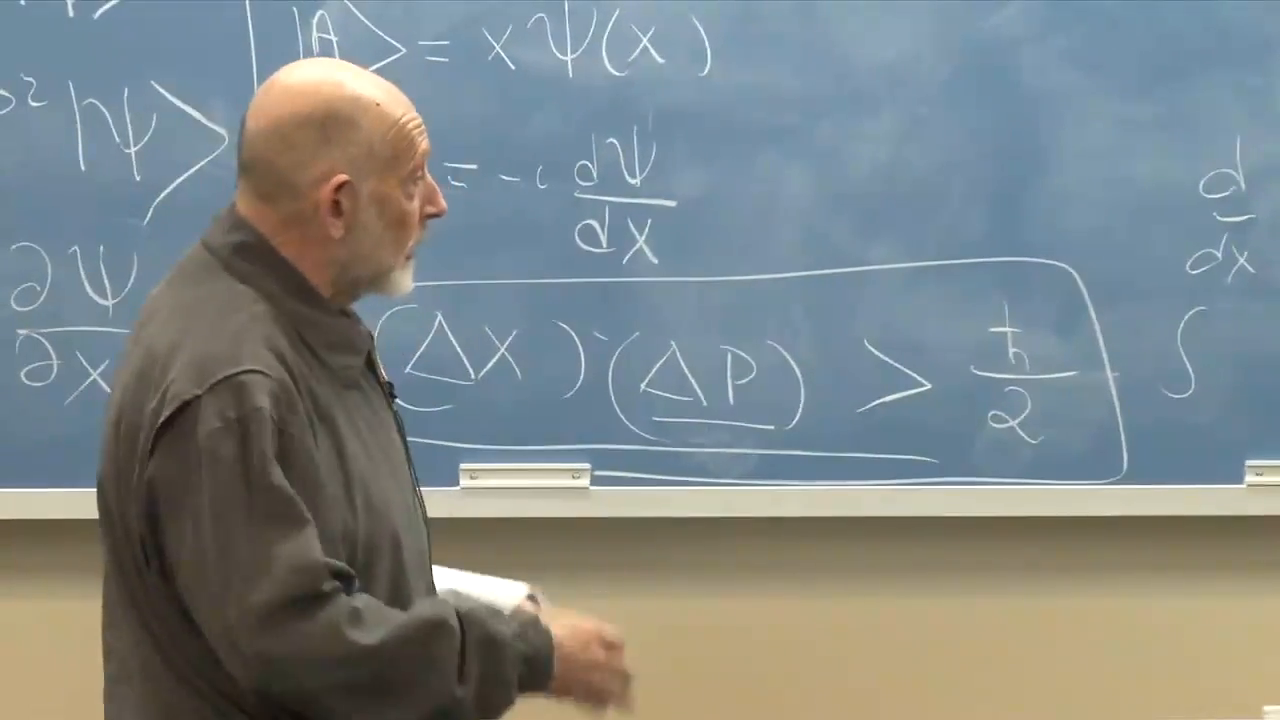
\includegraphics[width=0.88\textwidth]{lecture_10_figure_05.png}
\caption{부분적분을 하면 \(\expect{P^2}\)의 겉보기 음수 표현이 명백히 양수인 노름으로 바뀐다.}
\lectureframe{00:27:35}
\end{figure}

\begin{classroomqa}
\audiencequestion{위치와 운동량의 평균을 동시에 영으로 옮길 수 있나요?}
\lecturerresponse{네. 파동함수의 인자를 평행이동하면 \(\expect{X}\)가 변하고, 파동함수에 평면파 위상을 곱하면 \(\expect{P}\)가 변합니다. 이 연산들은 각각의 분산은 바꾸지 않으면서 평균을 바꾸므로, 증명에서는 두 변수를 모두 평균이 영인 상태로 두어도 됩니다.}
\end{classroomqa}

\section{불확정성 하한}

필요한 수학적 도구는 코시--슈바르츠 부등식이다. 강의에서는 이를 기초적인 벡터 기하로 설명한다. 두 벡터의 내적은 두 벡터의 길이와 그 사이 각도의 코사인의 곱이므로, 그 절댓값은 두 벡터 길이의 곱을 넘을 수 없다. 힐베르트 공간 표기에서는
\begin{equation}
\braket{A}{A}\braket{B}{B}
\geq
\left|\braket{A}{B}\right|^2.
\label{eq:l10-cauchy-schwarz}
\end{equation}
이다. 이 부등식은 임의의 차원을 가진 실수 또는 복소수 벡터 공간에서 성립한다.

\begin{figure}[htbp]
\centering
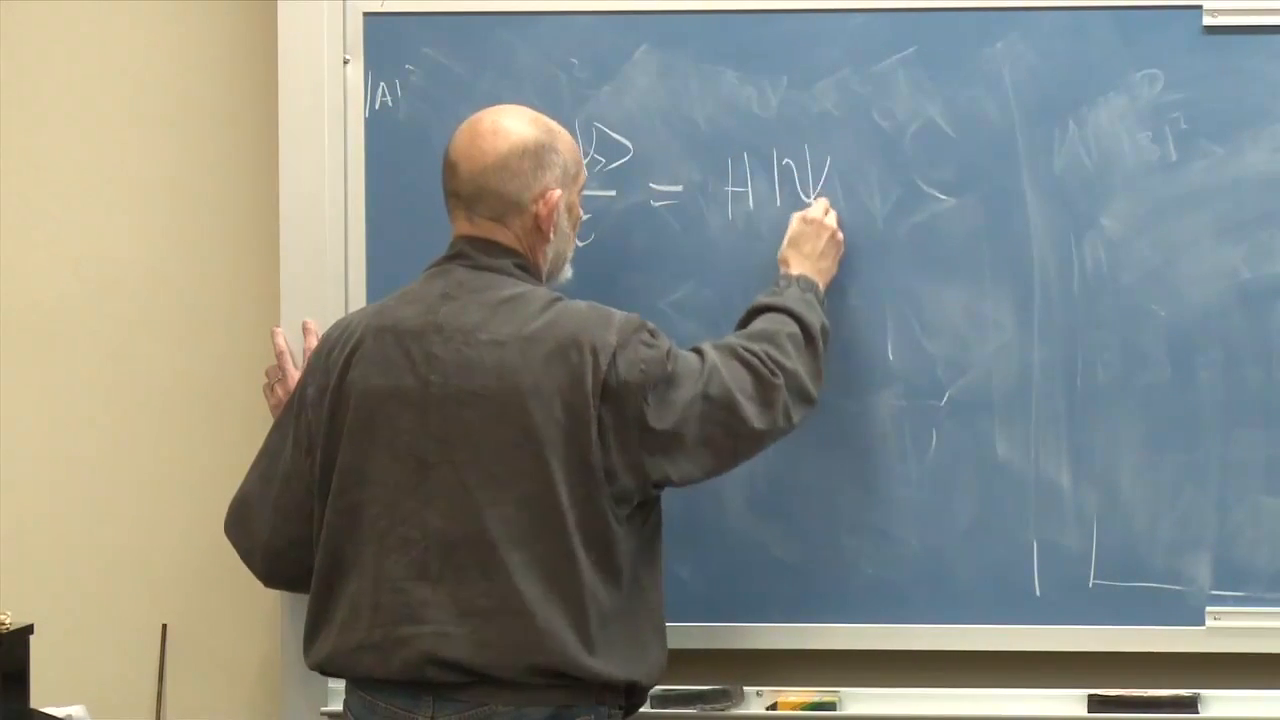
\includegraphics[width=0.88\textwidth]{lecture_10_figure_06.png}
\caption{기하학적 벡터 부등식은 증명에 쓰이는 힐베르트 공간의 코시--슈바르츠 부등식으로 다시 표현된다.}
\lectureframe{00:35:35}
\end{figure}

\begin{classroomqa}
\audiencequestion{부등식은 엄격한 부등호여야 하나요, 아니면 등호도 성립할 수 있나요?}
\lecturerresponse{크거나 같다는 관계다. 두 힐베르트 공간 벡터가 선형 종속이면 등호가 성립한다. 이 등호 조건을 이용하면 뒤에서 최소 불확정성 파동묶음을 알아낼 수 있다.}
\end{classroomqa}

두 변수의 평균을 모두 영으로 맞추고, 우선 \(\psi(x)\)가 실수라고 가정하는 칠판의 간략한 증명을 따라가자. 다음을 정의하자.
\begin{equation}
\ket{A}=X\ket{\psi},
\qquad
\ket{B}=P\ket{\psi}.
\label{eq:l10-auxiliary-vectors}
\end{equation}
이 벡터들의 노름의 제곱은 각각 정확히 분산이다.
\begin{equation}
\braket{A}{A}=(\Delta x)^2,
\qquad
\braket{B}{B}=(\Delta p)^2.
\end{equation}

\begin{figure}[htbp]
\centering
\includegraphics[width=0.88\textwidth]{lecture_10_figure_07.png}
\caption{보조 벡터 \(X\ket{\psi}\)와 \(P\ket{\psi}\)를 이용하면 두 분산을 힐베르트 공간 노름으로 나타낼 수 있다.}
\lectureframe{00:44:40}
\end{figure}

남은 내적은
\begin{align}
\braket{A}{B}
&=
\int_{-\infty}^{\infty}
dx\,
x\psi(x)
\left(-i\hbar\frac{d\psi}{dx}\right).
\end{align}
이다. 여기에는 그 절댓값만 들어간다. \(\psi\)가 실수이므로
\begin{equation}
\psi\frac{d\psi}{dx}
=
\frac{1}{2}\frac{d}{dx}\psi^2.
\end{equation}
이다. 따라서
\begin{align}
\left|\braket{A}{B}\right|
&=
\frac{\hbar}{2}
\left|
\int_{-\infty}^{\infty}
dx\,
x\frac{d}{dx}\psi^2
\right| \notag\\
&=
\frac{\hbar}{2}
\left|
-\int_{-\infty}^{\infty}
dx\,\psi^2
\right|
=
\frac{\hbar}{2},
\label{eq:l10-inner-product-half-hbar}
\end{align}
이다. 여기서는 부분적분으로 \(\psi^2\)에서 미분을 없애고, \(d x/dx=1\), 경계항은 사라지며, 정규화 조건으로 마지막 등식이 성립한다.

식~\eqref{eq:l10-inner-product-half-hbar}을 코시--슈바르츠 부등식에 대입하면
\begin{equation}
(\Delta x)^2(\Delta p)^2
\geq
\frac{\hbar^2}{4}.
\end{equation}
양의 제곱근을 취하면
\begin{equation}
\boxed{
\Delta x\,\Delta p
\geq
\frac{\hbar}{2}
}.
\label{eq:l10-uncertainty-principle}
\end{equation}

\begin{figure}[htbp]
\centering
\includegraphics[width=0.88\textwidth]{lecture_10_figure_08.png}
\caption{부분적분과 정규화 조건을 적용하면 위치-운동량 불확정성의 날카로운 하한을 얻는다.}
\lectureframe{00:50:55}
\end{figure}

\(\psi\)를 실수로 제한한 것은 칠판 위 증명을 간단히 하려는 편의였을 뿐, 정리의 적용 범위를 제한하는 조건이 아니다. 일반적인 복소 상태에서는 다음과 같이 둔다.
\begin{equation}
\ket{A}=(X-\expect{X})\ket{\psi},
\qquad
\ket{B}=(P-\expect{P})\ket{\psi}.
\end{equation}
교환자는 두 벡터의 겹침의 허수부를 정한다.
\begin{equation}
\operatorname{Im}\braket{A}{B}
=
\frac{1}{2i}\expect{[X,P]}
=
\frac{\hbar}{2}.
\end{equation}
\(|\braket{A}{B}|\)는 그 허수부의 절댓값보다 크거나 같으므로, 같은 하한이 따라 나온다.

\begin{classroomqa}
\audiencequestion{부분적분을 여러 번 할 때 경계항은 정확히 어떻게 처리되나요?}
\lecturerresponse{여기서 고려하는 정규화 가능한 파동묶음의 경우, \(+\infty\)와 \(-\infty\)에서 나타나는 곱은 사라집니다. 유한한 주기 구간에서는 양 끝점의 항들이 서로 상쇄됩니다. 이러한 조건이 성립하도록 연산자의 정의역을 정해야 합니다. 그렇지 않으면 이 형식적인 조작은 정당화되지 않습니다.}
\end{classroomqa}

\begin{classroomqa}
\audiencequestion{등호가 실제로 물리적으로 달성될 수 있나요, 아니면 하한은 단지 추정치인가요?}
\lecturerresponse{달성될 수 있다. 코시--슈바르츠 부등식에서 등호가 성립하려면 두 보조 벡터가 서로 비례해야 한다. 그 조건을 풀면 가우스 파동묶음이 나오며, 다음에 다룰 최소 불확정성 상태가 바로 이것이다.}
\end{classroomqa}

\section{다른 푸리에 켤레쌍}

시간과 에너지 사이의 불확정성 관계는 위치와 운동량 사이의 관계와 비슷하다. 그러나 여기서는 시간을 보통 보편적인 자기수반 연산자로 나타내는 관측량이 아니라 시간 발전의 매개변수로 쓰므로 더 주의해야 한다. 에너지 고유벡터를 사용해 상태를 전개하면
\begin{equation}
\ket{\psi(t)}
=
\int dE\,
\phi(E)e^{-iEt/\hbar}\ket{E}.
\label{eq:l10-time-energy-fourier}
\end{equation}
에너지 진폭과 시간에 따른 변화는 푸리에 관계를 이룬다. 에너지 분포의 폭이 좁으면 상태는 천천히 변하므로 시각이 뚜렷한 펄스를 만들 수 없다. 에너지 분포의 폭이 넓으면 짧은 도착 시간 포락선을 만들 수 있다.

\begin{figure}[htbp]
\centering
\includegraphics[width=0.88\textwidth]{lecture_10_figure_09.png}
\caption{에너지 고유상태에 위상 \(e^{-iEt/\hbar}\)를 곱해 시간 의존성을 구성하면 시간-에너지 관계의 푸리에 기저를 얻는다.}
\lectureframe{00:53:40}
\end{figure}

\begin{classroomqa}
\audiencequestion{시간과 에너지에도 같은 증명을 바로 적용할 수 있나요?}
\lecturerresponse{역수 관계에 관한 직관은 적용되며, 지나가는 파동묶음이 유용한 예를 제공한다. 짧은 도착 시간 구간을 만들려면 넓은 에너지 분포가 필요하다. 다만 이 정식화에서 시간은 \(X\)와 정확히 같은 방식으로 등장하지 않으므로, 연산자에 관한 진술은 더 미묘하다.}
\end{classroomqa}

각도와 각운동량도 회전 운동의 켤레쌍을 이룬다. 국소적으로 두 변수 사이의 푸리에 관계는 위치와 운동량의 관계와 비슷하다. 그러나 전역적으로는 각도의 주기성 때문에 추가로 주의할 점이 있으므로, 여기서 이 설명은 완전한 정리가 아니라 유비다.

\begin{classroomqa}
\audiencequestion{위치-운동량, 시간-에너지, 각도-각운동량은 고립된 몇 가지 예에 불과한가요?}
\lecturerresponse{아니다. 정준 켤레 변수는 푸리에 쌍으로 거듭 나타난다. 정의역과 주기성에 관한 세부 사항은 서로 다르지만, 국소화 폭이 서로 역수 관계를 이룬다는 것이 공통된 구조다.}
\end{classroomqa}

\section{Schr\"odinger 방정식의 위치 공간 표현}

이제 시간 발전으로 돌아가자. 추상적인 법칙은
\begin{equation}
i\hbar\frac{d}{dt}\ket{\psi(t)}
=
H\ket{\psi(t)}.
\label{eq:l10-abstract-schrodinger}
\end{equation}
질량이 \(m\)이고 퍼텐셜이 \(V(X)\)인 입자에 대해서는
\begin{equation}
H=\frac{P^2}{2m}+V(X).
\label{eq:l10-particle-hamiltonian}
\end{equation}
로 둔다. 이는 고전적인 운동 에너지와 퍼텐셜 에너지의 합이라는 형태를 가져온 뒤, 적절한 영역에서 양자 시간 발전이 고전 운동을 재현하는지 살펴보는 것이다.

\begin{figure}[htbp]
\centering
\includegraphics[width=0.88\textwidth]{lecture_10_figure_10.png}
\caption{시간 의존 Schr\"odinger 방정식에서 해밀토니안은 추상 상태 벡터에 작용한다.}
\lectureframe{00:59:05}
\end{figure}

위치 표현에서 \(P^2\)는 2차 미분 연산자가 된다. \(X\)의 함수는 곱셈으로 작용한다.
\begin{equation}
\bigl(V(X)\psi\bigr)(x)=V(x)\psi(x).
\end{equation}
따라서
\begin{equation}
i\hbar\frac{\partial\psi(x,t)}{\partial t}
=
\left[
-\frac{\hbar^2}{2m}\frac{\partial^2}{\partial x^2}
+V(x)
\right]\psi(x,t).
\label{eq:l10-position-schrodinger}
\end{equation}

\begin{figure}[htbp]
\centering
\includegraphics[width=0.88\textwidth]{lecture_10_figure_11.png}
\caption{입자의 해밀토니안은 운동 에너지에 해당하는 2차 미분 항과 \(V(x)\)를 곱하는 항으로 표현된다.}
\lectureframe{01:03:05}
\end{figure}

\begin{classroomqa}
\audiencequestion{통상적인 함수 \(V(x)\)는 어떤 의미에서 연산자인가요?}
\lecturerresponse{위치 기저를 선택하면 \(X\)는 \(x\)를 곱하는 방식으로 작용한다. 따라서 충분히 매끄러운 함수 \(V(X)\)는 각 점에서 해당하는 수 \(V(x)\)를 곱하는 방식으로 작용한다. 그 유용성은 뒤이어 나오는 시간 발전으로 확인한다.}
\end{classroomqa}

기댓값을 계산하기 위해 식~\eqref{eq:l10-position-schrodinger}에서 두 시간 미분을 구하면
\begin{align}
\dot{\psi}
&=
\frac{i\hbar}{2m}\psi''
-\frac{i}{\hbar}V\psi,
\label{eq:l10-psi-dot}\\
\dot{\psi}^{\,*}
&=
-\frac{i\hbar}{2m}\psi^{*\,\prime\prime}
+\frac{i}{\hbar}V\psi^*.
\label{eq:l10-psi-star-dot}
\end{align}
두 번째 줄은 첫 번째 줄의 복소켤레일 뿐이지만, 두 식을 모두 쓰면 상쇄되는 항이 눈에 잘 보인다.

\section{파동묶음 중심의 운동}

위치 분포의 중심은
\begin{equation}
\expect{X}
=
\int_{-\infty}^{\infty}
dx\,\psi^*(x,t)\,x\,\psi(x,t).
\end{equation}
이다. 이를 미분하면
\begin{equation}
\frac{d}{dt}\expect{X}
=
\int dx\,
\left(
\dot{\psi}^{\,*}x\psi
+
\psi^*x\dot{\psi}
\right).
\label{eq:l10-x-expectation-derivative}
\end{equation}
두 항은 서로 복소켤레다. 식~\eqref{eq:l10-psi-dot}와 \eqref{eq:l10-psi-star-dot}를 대입하면 \(V(x)\)가 실수이므로 퍼텐셜 항들이 상쇄된다. 운동 에너지 항에 부분적분을 적용하면
\begin{align}
\frac{d}{dt}\expect{X}
&=
\frac{1}{m}
\int dx\,
\psi^*
\left(-i\hbar\frac{\partial}{\partial x}\right)
\psi \notag\\
&=
\frac{\expect{P}}{m}.
\label{eq:l10-ehrenfest-x}
\end{align}

\begin{figure}[htbp]
\centering
\includegraphics[width=0.88\textwidth]{lecture_10_figure_12.png}
\caption{파동묶음 중심의 미분은 운동량을 질량으로 나눈 값의 기댓값으로 환원된다.}
\lectureframe{01:15:40}
\end{figure}

이 관계는 정확하다. 계산 과정에 좁은 파동묶음 근사는 전혀 들어가지 않았다.

\begin{classroomqa}
\audiencequestion{이 유도 과정에서 파동묶음이 폭이 좁은 단일 봉우리라는 가정은 어디에 쓰였나요?}
\lecturerresponse{쓰이지 않았다. 항등식 \(d\expect{X}/dt=\expect{P}/m\)는 이 해밀토니안의 정의역에 속하는 모든 상태에서 성립한다. 국소화가 필요한 것은 \(\expect{X}\)를 고전 입자의 궤적으로 해석할 때뿐이다.}
\end{classroomqa}

역학의 나머지 절반은 운동량에 관한 것이다.
\begin{equation}
\expect{P}
=
\int dx\,
\psi^*
\left(-i\hbar\frac{\partial}{\partial x}\right)
\psi.
\end{equation}
시간에 의존하는 두 인자를 모두 미분하면
\begin{equation}
\frac{d}{dt}\expect{P}
=
-i\hbar
\int dx\,
\left(
\dot{\psi}^{\,*}\psi'
+
\psi^*\frac{\partial\dot{\psi}}{\partial x}
\right).
\label{eq:l10-p-expectation-start}
\end{equation}
항 하나에 부분적분을 적용한 뒤 두 Schr\"odinger 방정식을 대입한다. 운동 에너지 기여분은 상쇄된다. 퍼텐셜 항은 다음처럼 합쳐진다.
\begin{equation}
\int dx\,
V(x)
\left(
\psi\frac{\partial\psi^*}{\partial x}
+
\psi^*\frac{\partial\psi}{\partial x}
\right)
=
\int dx\,
V(x)\frac{\partial}{\partial x}|\psi|^2.
\end{equation}
마지막으로 한 번 더 부분적분하여 미분을 퍼텐셜에 옮기면
\begin{align}
\frac{d}{dt}\expect{P}
&=
-\int dx\,|\psi(x,t)|^2\frac{dV}{dx} \notag\\
&=
-\expect{V'(X)}
\\
&=
\expect{F(X)},\\
F(x)&=-V'(x).
\label{eq:l10-ehrenfest-p}
\end{align}

\begin{figure}[htbp]
\centering
\includegraphics[width=0.88\textwidth]{lecture_10_figure_13.png}
\caption{퍼텐셜 항들이 완전미분으로 합쳐져 \(d\expect{P}/dt=-\expect{V'(X)}\)를 얻는다.}
\lectureframe{01:30:45}
\end{figure}

식~\eqref{eq:l10-ehrenfest-x}와 \eqref{eq:l10-ehrenfest-p}는 이 해밀토니안에 대한 에렌페스트 정리다. 이들은 정확한 양자역학적 항등식이지만, 정확한 기댓값 방정식이 곧 고전 궤도를 뜻하는 것은 아니다.

\section{고전적 근사가 들어가는 곳}

파동묶음 중심에 있는 점입자에 대한 고전역학이라면 다음을 요구할 것이다.
\begin{equation}
\frac{d}{dt}\expect{P}
\approx
F\!\left(\expect{X}\right).
\label{eq:l10-classical-center-force}
\end{equation}
반면 양자역학이 주는 것은
\begin{equation}
\frac{d}{dt}\expect{P}
=
\expect{F(X)}.
\end{equation}
이다. 일반적으로는
\begin{equation}
\expect{F(X)}
\neq
F\!\left(\expect{X}\right).
\label{eq:l10-force-nonlinearity}
\end{equation}

\begin{classroomqa}
\audiencequestion{에렌페스트 방정식이 둘 다 정확하다면, 왜 모든 양자 상태가 뉴턴 법칙을 따른다는 것을 이미 증명하지 못하나요?}
\lecturerresponse{파동묶음 중심에 뉴턴 법칙을 적용하려면 중심에서 힘을 계산해야 한다. 정확한 양자 방정식에는 전체 확률분포에 걸쳐 평균한 힘이 들어간다. 파동묶음이 좁고 힘장이 천천히 변하는 경우에는 두 값이 일치하지만, 임의의 상태나 비선형적인 힘에서는 그렇지 않다.}
\end{classroomqa}

강의의 반례는 이 차이를 분명히 보여 준다. \(F(x)=x^2\)라 하고, \(+a\)와 \(-a\) 근처에 폭이 좁은 봉우리 두 개가 같은 크기로 있는 정규화 상태를 택하자. 대칭성으로부터
\begin{equation}
\expect{X}=0,
\qquad
F\!\left(\expect{X}\right)=0,
\end{equation}
이지만
\begin{equation}
\expect{F(X)}
=
\expect{X^2}
\approx
a^2>0.
\end{equation}

\begin{figure}[htbp]
\centering
\includegraphics[width=0.88\textwidth]{lecture_10_figure_14.png}
\caption{대칭인 두 봉우리 파동묶음에서 \(F(x)=x^2\)일 때, 평균 위치에서의 힘은 사라지지만 평균 힘은 사라지지 않는다.}
\lectureframe{01:33:35}
\end{figure}

\(\bar{x}=\expect{X}\)를 중심으로 한 폭이 좁은 단일 파동묶음에 대해 힘을 전개하면
\begin{equation}
F(X)
=
F(\bar{x})
+
F'(\bar{x})(X-\bar{x})
+
\frac{1}{2}F''(\bar{x})(X-\bar{x})^2
+\cdots.
\end{equation}
기댓값을 취하면 일차항은 사라진다.
\begin{equation}
\expect{F(X)}
=
F(\bar{x})
+
\frac{1}{2}F''(\bar{x})(\Delta x)^2
+\cdots.
\end{equation}
힘이 눈에 띄게 변하는 길이 척도에 비해 파동묶음이 계속 좁게 유지될 때 고전적 근사가 타당하다.

날카로운 구조는 파동묶음을 분할하고 산란시킬 수 있다. 넓고 매끄러운 퍼텐셜은 충분히 국소화된 파동묶음을 단일 봉우리 형태로 유지하면서 유도하는 경향이 있다. 반면 점과 같은 장애물, 원자핵, 또는 파장과 비슷한 규모의 구조는 반사 성분과 회절 성분을 만들어 낼 수 있다.

\begin{figure}[htbp]
\centering
\includegraphics[width=0.88\textwidth]{lecture_10_figure_15.png}
\caption{파동묶음 폭이나 관련 파장보다 짧은 척도의 퍼텐셜 구조는 결맞은 파동묶음을 산란 성분들로 분해할 수 있다.}
\lectureframe{01:37:25}
\end{figure}

\begin{classroomqa}
\audiencequestion{어떤 퍼텐셜이 고전적 파동묶음에 부적합한가요?}
\lecturerresponse{핵심은 도덕적 성격이 아니라 척도다. 파동묶음보다 훨씬 날카롭거나 그 파장과 비슷한 규모의 구조는 파동의 성질을 드러내고 산란을 일으킨다. 퍼텐셜이 파동묶음의 폭에 걸쳐 천천히 변하면 그 영역에서 힘은 거의 일정하므로 중심은 고전 방정식을 따른다.}
\end{classroomqa}

질량도 중요하다. 최소 불확정성에 가까운 파동묶음에 대해서는
\begin{equation}
\Delta x\,\Delta v
\sim
\frac{\hbar}{2m}.
\end{equation}
질량이 크면 공간 폭을 작게 유지하면서 속력의 퍼짐은 크지 않게 할 수 있다. 따라서 무거운 물체는 거시적인 퍼텐셜을 지나가는 동안에도 뚜렷하게 국소화된 상태를 유지할 수 있다. 가벼운 입자는 미시적인 구조에 의해 더 쉽게 퍼지거나 회절한다. 이는 질량만으로 운동이 고전적인지를 결정한다는 주장이 아니라, 스케일링에 관한 논증이다.

\begin{classroomqa}
\audiencequestion{이런 의미에서 전자도 고전적으로 근사할 만큼 큰 계가 될 수 있나요?}
\lecturerresponse{그렇다. 외부장이 전자 파동묶음의 크기에 비해 매끄럽게 변하면 가능하다. 예를 들어 간격이 넓은 축전기 판 사이에서는 결맞은 파동묶음이 유용한 시간 동안 고전적 가속을 따를 수 있다. 핵의 급격한 쿨롱 구조 근처에서는 같은 전자도 뚜렷한 산란을 보인다.}
\end{classroomqa}

러더퍼드의 1911 산란 실험은 상호보완적인 교훈을 준다. 금 원자의 조밀한 전하 분포와 만난 알파 입자는 큰 각도로 산란되었으며, 이로써 양전하가 매우 작은 영역에 집중되어 있음이 드러났다. 러더퍼드는 입자 빔으로 설명했고, 양자역학에서는 입사 진폭과 그 산란 성분으로 설명한다. 현대의 전자 및 광자 산란 실험도 같은 스케일 민감성을 이용한다.

\begin{classroomqa}
\audiencequestion{이 파동과 스케일의 관계는 물질 입자에만 해당하나요?}
\lecturerresponse{아니다. 굴절률이 파장에 걸쳐 천천히 변하면 전자기파는 기하광학의 법칙을 따른다. 간격이 파장과 비슷한 회절 격자는 파동을 뚜렷하게 구분되는 방향들로 퍼뜨린다. 전자, 알파 입자, 광자와 다른 양자 들뜸도 파장과 구조 사이의 같은 관계를 따른다.}
\end{classroomqa}

따라서 고전적 극한은 양자역학 위에 별도의 법칙을 덧붙인 것이 아니다. 정확한 기댓값 방정식에는 이미 고전적 관계가 들어 있다. 상태가 국소화된 채로 유지되고 해밀토니안이 충분히 매끄럽게 변해 힘의 평균과 파동묶음 중심에서 계산한 힘이 사실상 같아질 때 고전 궤도가 나타난다.
